\documentclass[sigconf, nonacm]{acmart}

\setcopyright{none}
\settopmatter{printacmref=false, printccs=false, printfolios=true}
\acmDOI{}
\acmISBN{}
\acmConference[PRISMA '26]{PRISMA Summer School}{June 15--19, 2026}{Geneva}

\usepackage{amsmath,amsfonts}
\usepackage{booktabs}
\usepackage{siunitx}
\usepackage{graphicx}
\graphicspath{{../figures/}{figures/}}
\sisetup{per-mode=symbol, group-separator={,}}

% --- compact float spacing to fit two pages ---
\setlength{\textfloatsep}{3pt plus 2pt minus 2pt}
\setlength{\intextsep}{3pt plus 2pt minus 2pt}
\setlength{\abovecaptionskip}{2pt}
\setlength{\belowcaptionskip}{0pt}

\begin{document}

\title{Net-zero CO$_2$ by 2070 in the SCI ensemble:\\ what a 2010--2025 hindcast can and cannot tell us}

\author{Lucas Alvarez}
\email{lualpi@upv.es}
\affiliation{\institution{Universitat Polit\`ecnica de Val\`encia}}

\author{Matteo Catania}
\email{matteo.catania@polimi.it}
\affiliation{\institution{Politecnico di Milano}}

\author{R\'emi Paccou}
\email{remi.paccou@proton.me}
\affiliation{\institution{CIRED, Nogent-sur-Marne}}
\affiliation{\institution{Schneider Electric, Grenoble}}

\begin{abstract}
Of the 1{,}564 pathways in the Scenario Compass Initiative (SCI) 2025 ensemble, 497 reach net-zero CO$_2$ by 2070, a naive frequency $P(\text{NZ2070})\approx 32\%$. We ask what the observed 2010--2025 record establishes about that figure. First, each pathway is a \emph{conditional} forecast (an outcome given an assumed policy path), so the count is a sample frequency, not a probability; it moves between 16\% and 57\% with the chosen deadline and between 24\% and 39\% with the team-weighting, neither of which is a climate quantity. Second, scoring the ensemble against observations for six variables, it sits below observed 2025 emissions ($+2{,}582$~Mt~CO$_2$/yr, family-weighted), the shortfall is concentrated in net-zero pathways, and a trivial extrapolation beats it on the variables that stayed on trend. The ensemble under-projects emissions, and the world is in an \emph{addition} regime: solar capacity roughly double the ensemble median while coal set a record. Conditioning on historical accuracy yields net-zero shares near 20\%, a sensitivity, not a revised probability. Independently, Wright's-law cost projections collapse alike for both groups, locating the binding constraint in fossil substitution, not the cost of clean generation. None of the shares reported here is an unconditional probability of net-zero by 2070.
\end{abstract}

\keywords{hindcast, scenario ensemble, net zero, conditional forecast, integrated assessment models}

\maketitle

% ============================================================================
\section{Introduction}
% ============================================================================
The SCI 2025 ensemble assembles 1{,}564 IAM pathways from 65 models across 41 research projects. Counting the 497 that reach net-zero CO$_2$ by 2070 gives $P(\text{NZ2070})\approx 32\%$. This count treats all pathways as equally credible draws from the future. We test that in two ways --- what the number \emph{is} (Sec.~\ref{sec:count}), and whether the ensemble behaves like a usable forecast on the recent past (Sec.~\ref{sec:hindcast}) --- then ask what a 15-year record can settle about a 45-year question (Sec.~\ref{sec:forecast}). We do not propose a corrected probability; we report where the evidence is firm.

% ============================================================================
\section{Data and method}
\label{sec:method}
% ============================================================================
We compare SCI-2025 (v1.0, global) projections at $t\in\{2010,2015,2020,2025\}$ with observed values for six variables: CO$_2$ emissions \cite{gcb}, coal primary energy \cite{ei}, solar PV and wind capacity \cite{irena}, nuclear capacity (IAEA PRIS), and GDP (PPP, World Bank). For pathway $j$, variable $v$, year $t$, the forecast error is $\varepsilon_{j,v,t}=y_{v,t}-\hat{y}_{j,v,t}$ ($\varepsilon>0$: the pathway projected too little). We summarise it by mean error ME (bias), MAE (typical magnitude), and RMSE. A pathway is \emph{net-zero-by-2070} if its SCI year-of-net-zero (CO$_2$) is $\leq 2070$. Three further statistics enter below: \emph{skill} $=|\varepsilon_{\text{ens}}|/|\varepsilon_{\text{rule}}|$ against a naive 2010--2015 random-walk or trend rule ($>1$: the rule wins); \emph{calibration}, the percentile (PIT) at which the observed value falls in the ensemble cloud; and a \emph{credibility filter} keeping the lowest-MAE quartile on the selected variables. Because the ensemble is a convenience sample (five families contribute about two-thirds of the runs), we weight each pathway by $1/n_f$ (its family size) and check scenario- and project-weighting. This is a \emph{hindcast} (a backtest on a window each model could see), not an out-of-sample test: all pathways post-date 2017.

% ============================================================================
\section{The naive count is a sample frequency, not a probability}
\label{sec:count}
% ============================================================================
A pathway states $\hat{y}=f(P)$: an outcome \emph{given} an assumed policy/technology path $P$. Counting conditional ``if--then'' statements does not yield an unconditional probability, and the count is elastic to choices unrelated to the climate. Two such degrees of freedom each move it by roughly half its range (Table~\ref{tab:sens}): the net-zero \emph{deadline}, and the \emph{weighting} that decides how many runs each team contributes. A quantity this sensitive to arbitrary conventions is not estimating a probability. We therefore stop revising the number and instead test the ensemble as a forecast.

\begin{table}[h]
\centering\small
\caption{The net-zero share moves with two non-climate choices.}
\label{tab:sens}
\begin{tabular}{lcccc}
\toprule
\textbf{Deadline} & 2060 & 2070 & 2080 & ever ($\leq$2100) \\
Share & 16\% & 31\% & 43\% & 57\% \\
\midrule
\textbf{Weighting} & \multicolumn{2}{c}{per scenario} & per family & per project \\
Share (2070) & \multicolumn{2}{c}{31\%} & 24\% & 39\% \\
\bottomrule
\end{tabular}
\end{table}

% ============================================================================
\section{Hindcast diagnosis}
\label{sec:hindcast}
% ============================================================================
\paragraph{The 2025 undershoot is structural.}
Family-weighted CO$_2$ errors are $+405$ (2010), $+15$ (2015), $-1{,}572$ (2020), $+2{,}582$~Mt/yr (2025). The 2020 overshoot is mostly the COVID dip: replacing 2020 by a shock-free interpolation removes about three-quarters of it. The 2025 shortfall is not an artefact --- observed emissions lie on the pre-COVID trend, while the ensemble assumed an earlier peak-and-decline (Fig.~\ref{fig:overview}). It survives detrending.

\begin{figure}[t]
\centering
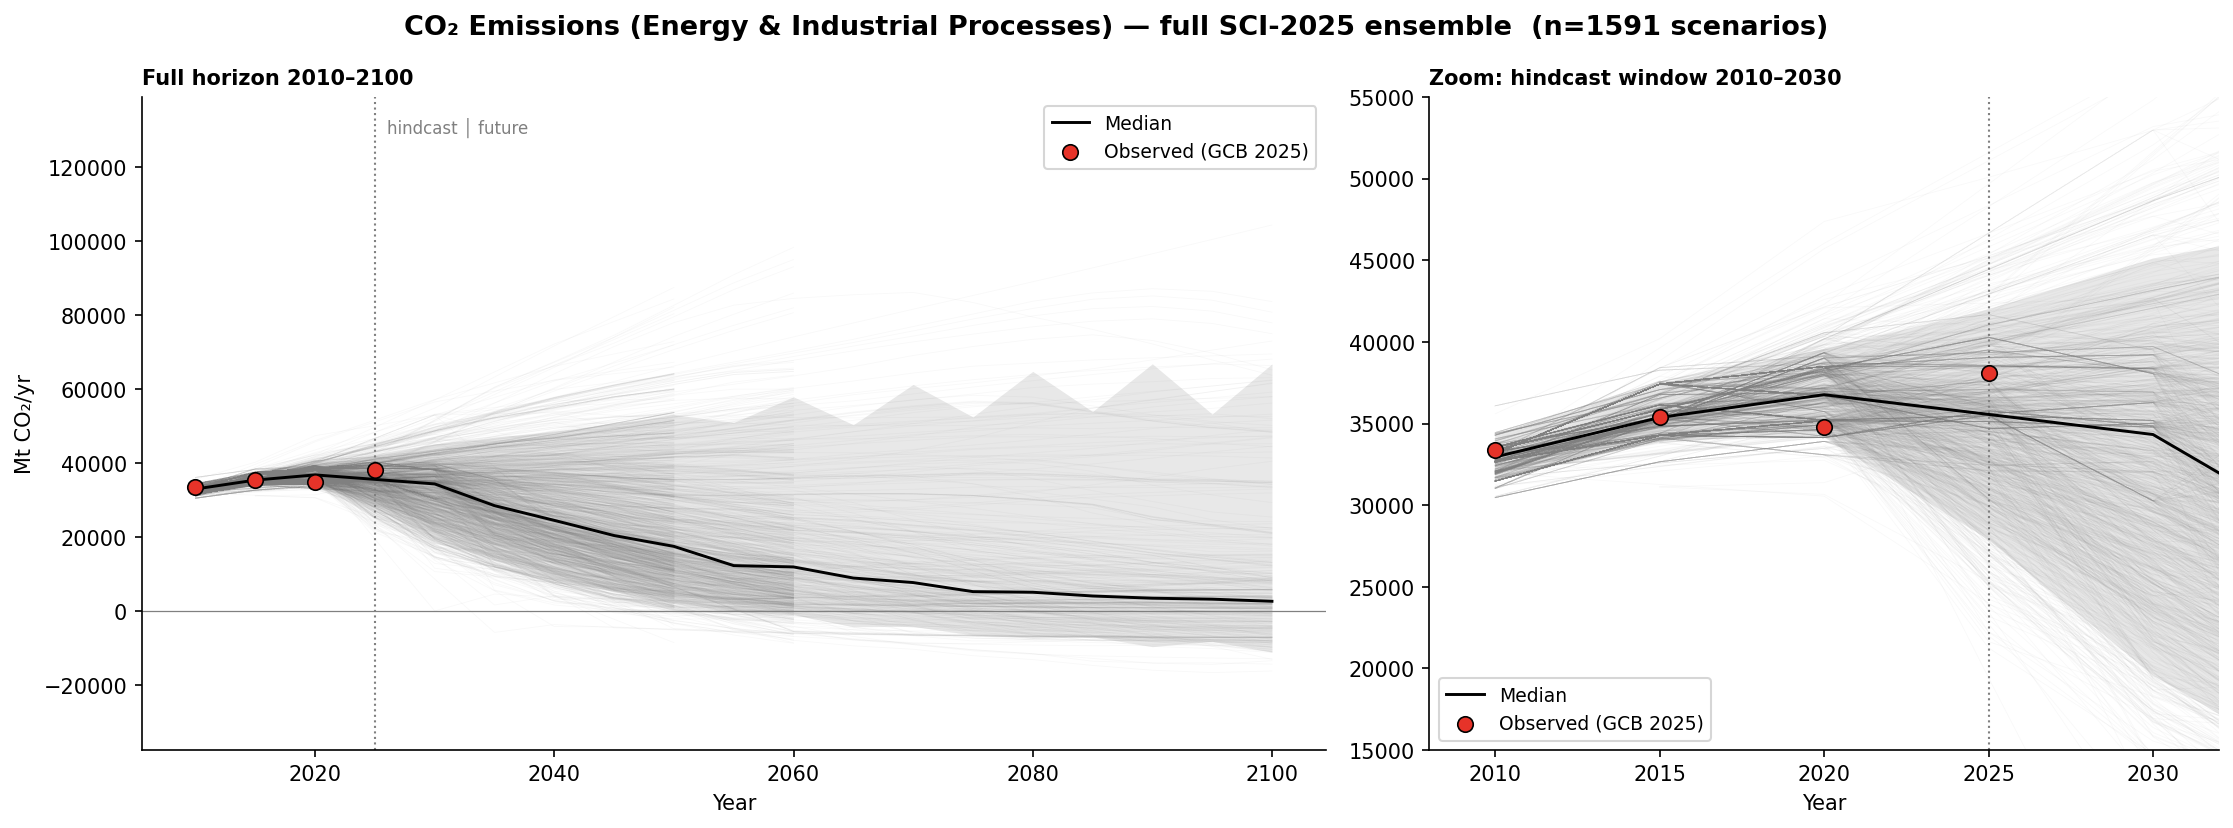
\includegraphics[width=\linewidth]{co2_overview}
\caption{The SCI CO$_2$ ensemble (grey) and the four observed points (black). Observed 2025 emissions sit above the ensemble central tendency.}
\label{fig:overview}
\end{figure}

\paragraph{The shortfall is concentrated in net-zero pathways.}
Mean error by outcome is $+650$ (net-zero) versus $+216$~Mt/yr (non-net-zero), family-weighted. The non-net-zero \emph{level} is weighting-dependent (near zero under scenario-weighting), so we read the \emph{gap}, which is robust ($+434$, $+837$, $+1{,}281$ under family/scenario/project weighting). Typical magnitudes are close (MAE $\approx 6\%$ vs $5\%$): a directional bias, not greater imprecision. Recent projects (post-2021) are better calibrated at their base year but undershoot 2025 more ($+3{,}280$ vs $+466$ for pre-2017), reflecting increasingly ambitious policy assumptions rather than improved skill.

\paragraph{No skill against a ruler on the on-trend variables.}
Forecasting 2025 from 2010--2015 with a random walk or linear trend, the rule beats the ensemble on 4 of 6 variables (skill: CO$_2$~2.0, coal~4.7, GDP~3.0, nuclear~9.9), and loses only where deployment accelerated (solar~0.7, wind~0.6) --- the same fact as the bias: the rule wins because reality stayed on trend while the ensemble bet on a turn.

\paragraph{Reality is off-centre in the cloud.}
The percentile of observed 2025 (the share of scenarios \emph{below} it) is 1st (GDP), 20th (nuclear), 75th (CO$_2$), 75th (wind), 79th (coal), 90th (solar): the ensemble projected too little CO$_2$, coal and solar (reality high) and too much GDP and nuclear (reality low). With one point per variable this is a diagnostic of the low emissions bias, not a formal calibration test; ``overconfident'' is firm only for solar and GDP. Either way reality is rarely near the median, so the ensemble is not a clean distribution to read $P(\text{NZ2070})$ from.

\paragraph{Addition, not substitution.}
Models underestimate fossil \emph{and} renewable deployment at once: 2025 solar (2{,}392~GW) is about double the ensemble median (1{,}169~GW), yet coal set a record (164~EJ). Coal and solar errors are anti-correlated ($\rho=-0.28$; $-0.30$ for net-zero): the pathways embed a substitution logic, but the world adds renewables on top of persistent fossils.

\paragraph{Which variables carry the signal.}
Separation $(\text{med}_{\text{NZ}}-\text{med}_{\text{non}})/\text{IQR}$ is appreciable only for coal ($+0.46$), CO$_2$ ($+0.39$) and solar ($-0.32$), confirmed by a LASSO classifier; the signs disagree (net-zero worse on coal/CO$_2$, better on solar), so credibility must be filtered jointly, not on CO$_2$ alone.

\paragraph{Filtering: a sensitivity, not a revision.}
Keeping the most accurate quartile and recomputing the share gives about 20\% (CO$_2$ filter), 22\% (joint coal+CO$_2$+solar), and 48\% (solar-only) against a $\sim$32\% baseline. The robust feature is the \emph{dependence} on the conditioning variable, which is exactly the conditional-forecast point of Sec.~\ref{sec:count}: no single unconditional share exists. We report $\sim$20\% under sensible criteria as a sensitivity floor; the 48\% arises only from filtering on solar, the variable every model misses.

% ============================================================================
\section{What a 15-year record cannot settle, and what it can}
\label{sec:forecast}
% ============================================================================
A backtest over 15 years cannot resolve a 45-year question: for a drifting random walk the error variance grows as $\sigma^2(\tau+\tau^2/m)$ in the horizon $\tau$. A pathway that stays flat to $\sim$2030 then falls steeply to net-zero is indistinguishable from a non-net-zero pathway over 2010--2025, so filtering cannot push below the late-mover share ($\sim$20\% acts as a practical, not a proven, floor). One quantity does carry skill: technology cost. Solar PV fell from $\sim$2{,}440 to $\sim$250~USD/kW (2010--2024); a Wright's-law fit (cost $\propto$ cumulative-capacity$^{-b}$, learning rate $\approx 0.39$, projected along each group's capacity path) gives $\sim$40~USD/kW by 2070, with a $\pm 2$~s.e.\ learning-rate band that overlaps across groups, and the net-zero and non-net-zero projections nearly coincide (Fig.~\ref{fig:wright}). Generation cost is therefore not the binding constraint --- clean technology is outperforming the scenarios whether or not the world reaches net-zero, though system costs (grids, storage, capital) still shape the rate. Reconciling the two halves: the ensemble is too optimistic on \emph{emissions} yet too pessimistic on \emph{cost}, because the world both deploys renewables faster than any model and keeps its fossils. The lock on net-zero is substitution, not primarily the price of clean generation.

\begin{figure}[t]
\centering
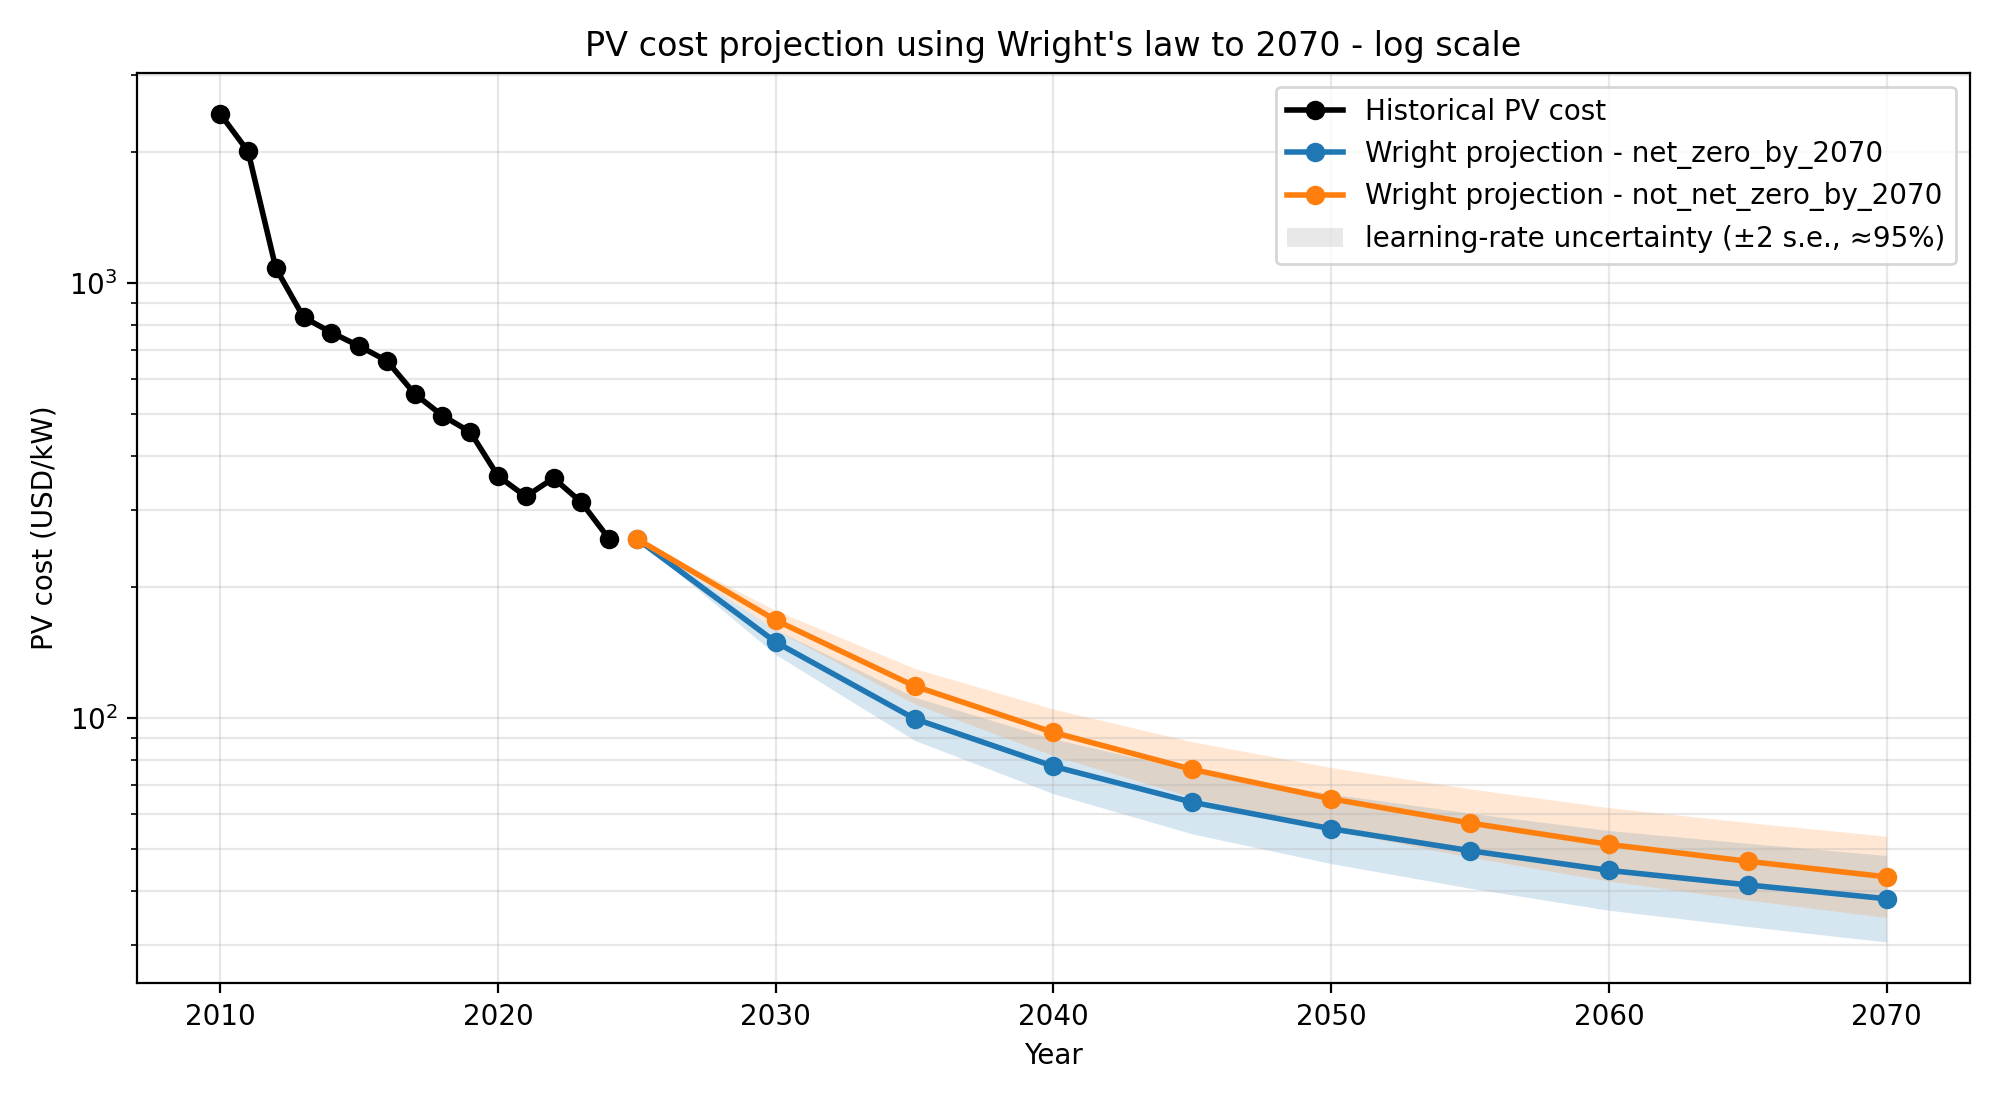
\includegraphics[width=0.88\linewidth]{pv_wright_cost_projection_to_2070_log}
\caption{Wright's-law PV cost projection to 2070 (log scale). Net-zero and non-net-zero trajectories nearly coincide; shading is the $\pm 2$ s.e.\ learning-rate band, which overlaps across the two groups.}
\label{fig:wright}
\end{figure}

% ============================================================================
\section{Conclusion}
% ============================================================================
None of this forecloses net-zero by 2070; it relocates the constraint. The naive 32\% is a sample frequency, not a probability; the record gives no support for reading the count as an unconditional probability; credibility filtering gives a sensitivity centred near 20\% that cannot be sharpened with a 15-year window. The decisive variable is substitution --- policy and system inertia retiring fossils --- not primarily the cost of clean generation (system costs still shape the rate). Three caveats bound these claims: 2020--2025 contains the COVID shock and rebound, which no pathway was built to capture; all pathways post-date 2017, so this is a hindcast, not a true out-of-sample test; and the calibration evidence rests on one observed point per variable. Within those bounds, the cross-model optimism about fossil phase-out points to a structural feature of the ensemble rather than a transient one.

\bibliographystyle{ACM-Reference-Format}
\begin{thebibliography}{6}
\setlength{\itemsep}{0pt}\setlength{\parsep}{0pt}
\bibitem{gcb} Friedlingstein, P. et al. (2026). Global Carbon Budget 2025. \emph{ESSD}, 18.
\bibitem{ei} Energy Institute (2025). \emph{Statistical Review of World Energy 2025}.
\bibitem{irena} IRENA (2026). \emph{Renewable Capacity Statistics 2026}. Abu Dhabi.
\bibitem{farmer} Farmer, J.D.\ \& Lafond, F. (2016). How predictable is technological progress? \emph{Research Policy}, 45(3), 647--665.
\bibitem{way} Way, R.\ et al. (2022). Empirically grounded technology forecasts and the energy transition. \emph{Joule}, 6(9), 2057--2082.
\bibitem{sci} Scenario Compass Initiative, \url{https://scenariocompass.org}.
\end{thebibliography}

\end{document}
